\begin{description}
    \item[Problem Statement:]
        Compute $fib(n)$, the $n$'th number in the Fibonacci sequence. (Where $fib(1) = 1$, $fib(2) = 1$ and $fib(n) = fib(n-1) + fib(n-2)$.)
        
    \item[Input:] 
        A positive integer $n$.
        
    \item[Output:] 
        An positive integer $fib(n)$.
        
    \item[Example:]
        For: 

        $n = 7$
        
        $fib(n) = 13$

    \item[Explanation:]
        The Fibonacci sequence is as follows: 1,1,2,3,5,8,13,...\\
        We can see that the 7th number in the sequence is 13.

\end{description}


\subsection{Brute Force Approach to Fib(n)}

We will always start with a brute force approach, in which which will use recursion to explore all subproblems and arrive at the solution. 
We know that the base cases are $fib(1) = 1$ and $fib(2) = 1$.
By definition, we know that the recursive case is $fib(n) = fib(n-1) + fib(n-2)$.

A sample Python implementation is shown in Figure \ref{fig:fibonacci-bf}.

\begin{figure}[H]
    \centering
    \begin{lstlisting}
    def fib_bf(n):
        if n <=2: return 1
        return fib_bf(n-1) + fib_bf(n-2)
    \end{lstlisting}
    \caption{Fibonacci Brute Force Python Implementation}
    \label{fig:fibonacci-bf}
\end{figure}

In order to understand just how inefficent this approach is, consider the calculation of $fib(6)$.
Figure \ref{fig:fibonacci-bf-tree} shows the repeating subproblems, which share a color in the tree.
We can see that the amount of repeating subproblems would scale exponentially with $n$.

\begin{figure}[htbp]
    \centering
    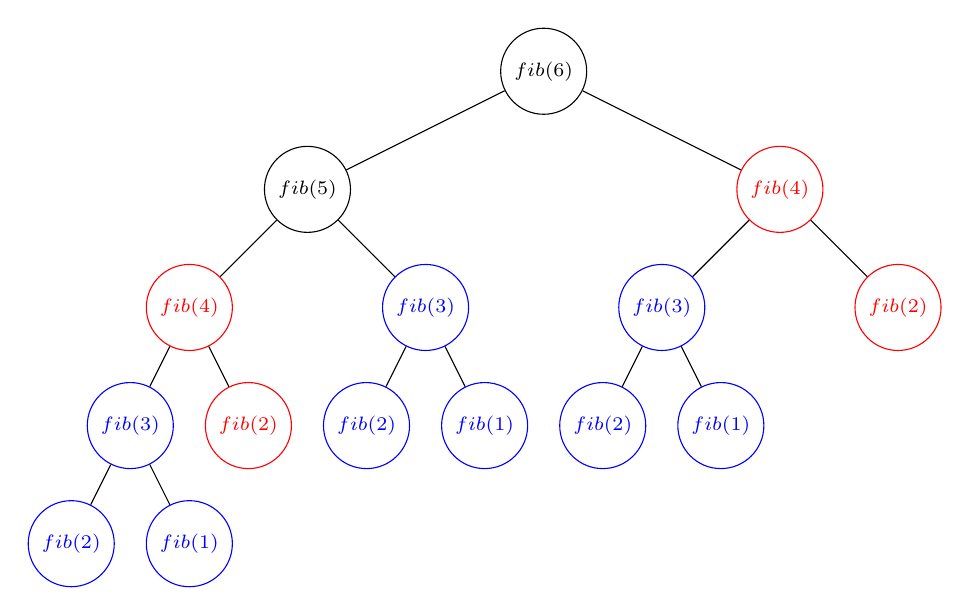
\begin{tikzpicture}[
        every node/.style={circle,draw,font=\scriptsize}, % Smaller font size
        level 1/.style={sibling distance=6cm},
        level 2/.style={sibling distance=3cm},
        level 3/.style={sibling distance=1.5cm}
    ]
        \node {$fib(6)$}
        child {node {$fib(5)$}
            child {node[red] {$fib(4)$}
                child {node[blue] {$fib(3)$}
                    child {node[blue] {$fib(2)$}}
                    child {node[blue] {$fib(1)$}}
                }
                child {node[red] {$fib(2)$}}
            }
            child {node[blue] {$fib(3)$}
                child {node[blue] {$fib(2)$}}
                child {node[blue] {$fib(1)$}}
            }
        }
        child {node[red] {$fib(4)$}
                child {node[blue] {$fib(3)$}
                    child {node[blue] {$fib(2)$}}
                    child {node[blue] {$fib(1)$}}
                }
                child {node[red] {$fib(2)$}}
            }
        ;
    \end{tikzpicture}
    
    \caption{Brute Force calculation of $fib(6) = 8$. Repeated subproblems share a color.}
    \label{fig:fibonacci-bf-tree}
\end{figure}

\subsection{Complexity Analysis of the Brute Force Approach to Fib(n)}

\begin{description}
    \item[Time Complexity:]
    At each step in the calculation of $fib(n)$, we make two 'branches', where one calculates $fib(n-1)$ and the other calculates $fib(n-2)$.
    This branching factor leads to an exponential growth in the number of function calls.
    The number of function calls grows exponentially with $n$, as each level of the tree doubles the number of function calls.
    Therefore the time complexity of this approach is $2 + 2^2 + 2^3 + ... + 2^n$ which is $O(2^n)$.
        
    \item[Space Complexity:] 
        In the brute force approach to The Fibonacci Problem, the space complexity is influenced by the recursive calls, each of which adds a frame to the call stack. However, as the recursion progresses, some of these frames can be discarded once their corresponding Fibonacci values have been computed.
        Specifically, at any point during the recursion, we only need to keep track of the previous two Fibonacci numbers. Therefore, the maximum depth of the call stack at any point is at most $n$ due to the recursion.
        This means that the space complexity of the brute force approach to compute Fibonacci numbers is $O(n)$.
        
        
    \item[Overall:] Total:\\
        Time Complexity: $O(2^n)$\\
        Space Complexity: $O(n)$
        
\end{description}
\newpage

\subsection{Memoization Approach to Fib(n)}
We can see that the optimal solution to $fib(n-1)$ + the optimal solution to $fib(n-2)$ will always be the optimal solution to $fib(n)$. This shows that the optimal substructure property holds.
We can also see that the calculation of $fib(n-1)$ contains the calculation of $fib(n-2)$, which is proof of overlapping subproblems.
This proves that the Fibonacci Problem fits the criteria for dynamic programming.
We can hence make this calculation more efficient through the use of memoization.
This simple adjustment involves storing a $(key, value)$ table called $memo$, where the key is an identifier for an intermediate subproblem and the value is the intermediate result of that subproblem.
Now, for any subproblem, we first check if the result is in $memo$ and if it is, we do not perform the calculation again, instead we return the result of that calculation from $memo$ in constant time.
If the subproblem is not in $memo$, we calculate the intermediate result and cache it in $memo$.

A sample Python implementation is shown in Figure \ref{fig:fibonacci-memo}.

\begin{figure}[H]
    \centering
    \begin{lstlisting}
    def fib_memo(n, memo={}):
        if n <= 2:
            return 1
        if n in memo:
            return memo[n]
        memo[n] = fib_memo(n-1, memo) + fib_memo(n-2, memo)
        return memo[n]
    \end{lstlisting}
    \caption{Fibonacci Memoization Python Implementation}
    \label{fig:fibonacci-memo}
\end{figure}

In the memoization solution, it is clear that we never repeat the calculation of a subproblem.
To visualize this, see Figure \ref{fig:fibonacci-memo-tree}, where repeated subproblems share a color.
We can see that we never repeat a calculation, as every time we visit a new node, we first check if it is present in $memo$, and if it is, we return the result immediately.
In this case, our $memo$ table key is $x$, and the value at $x$ returned is $fib(x)$.

\begin{figure}[H]
    \centering
    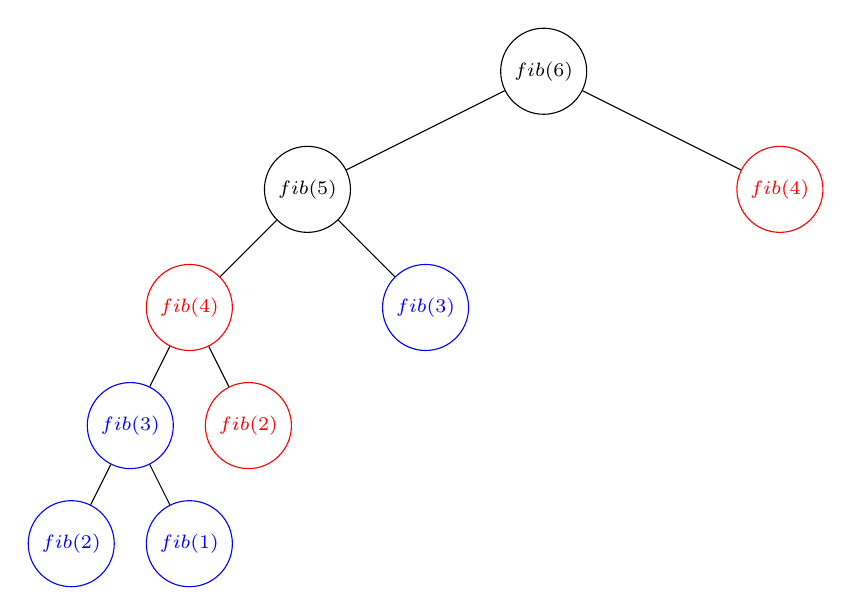
\begin{tikzpicture}[
        every node/.style={circle,draw,font=\scriptsize}, % Smaller font size
        level 1/.style={sibling distance=6cm},
        level 2/.style={sibling distance=3cm},
        level 3/.style={sibling distance=1.5cm}
    ]
        \node {$fib(6)$}
        child {node {$fib(5)$}
            child {node[red] {$fib(4)$}
                child {node[blue] {$fib(3)$}
                    child {node[blue] {$fib(2)$}}
                    child {node[blue] {$fib(1)$}}
                }
                child {node[red] {$fib(2)$}}
            }
            child {node[blue] {$fib(3)$}
            }
        }
        child {node[red] {$fib(4)$}
            }
        ;
    \end{tikzpicture}\\
    $memo$:
    \begin{table}[H]
        \centering
        \begin{tabular}{|c|c|c|c|c|c|c|}
            \hline
            \textbf{key:} & 1 & 2 & 3 & 4 & 5 & 6 \\
            \hline
            \textbf{value:} & 1 & 1 & 2 & 3 & 5 & 8 \\
            \hline
        \end{tabular}
    \end{table}
    \caption{Memoization calculation of $fib(6) = 8$. Repeated subproblems share a color.}
    \label{fig:fibonacci-memo-tree}
\end{figure}

\subsection{Complexity Analysis of the Memoization Approach to Fib(n)}

\begin{description}
    \item[Time Complexity:]
        Since each subproblem is only ever computed once, and any repeated subproblems are handled with a constant time table lookup,
        the time complexity depends only on the amount of subproblems.
        Since there are $n$ possible subproblems for any given input $n$,
        the time complexity is reduced to $O(n)$

    \item[Space Complexity:] 
        The space complexity remains determined by the recursion call stack, at $O(n)$.
        We also have to store the memo table, which contains an integer solution to each of the $n$ subproblems.
        This is also $O(n)$, giving us a total $O(2n)$ space complexity.
        This can be simplified to $O(n)$.

    \item[Overall:] Total:\\
        Time Complexity: $O(n)$\\
        Space Complexity: $O(n)$
        
\end{description}
\newpage

\subsection{Tabulation Approach to Fib(n)}
    
With the memoization approach, we saw how to compute the solution top-down, starting at $fib(n-1) + fib(n-2)$,
arriving at the base cases, and working up from there.
Notice that this step is unnecessary.
If we can deduce $fib(3)$ from $fib(2) + fib(1)$ (both of which are given in the base case),
and $fib(4)$ from $fib(3)$ and $fib(2)$,
we can work bottom-up until we arrive at $fib(n)$.
This is done by initializing an array of size $n$, placing 1 in the first and second cells as follows:
\begin{table}[H]
    \centering
    \begin{tabular}{|c|c|c|c|c|c|}
        \hline
        1 & 1 & \phantom{0} & \phantom{0} & \phantom{0} & \phantom{0} \\
        \hline
    \end{tabular}
\end{table}
And for each empty cell, filling it with the sum of the previous two cells.
This reduces the space complexity from $O(2n)$ to $O(n)$,
as all we need to do is store the table.
It is common practice to refer to the table as $dp$ in tabulation approaches.
Figure \ref{fig:fibonacci-dp-table} shows the complete $dp$ table.

\begin{figure}[H]
    \centering
    $dp$:
    \begin{table}[H]
        \centering
        \begin{tabular}{|c|c|c|c|c|c|}
            \hline
            1 & 1 & 2 & 3 & 5 & 8 \\
            \hline
        \end{tabular}
    \end{table}
    \caption{Tabulation Calculation of $fib(6)$.}
    \label{fig:fibonacci-dp-table}
\end{figure}

A sample Python implementation is shown in Figure \ref{fig:fibonacci-dp}.

\begin{figure}[H]
    \centering
    \begin{lstlisting}
    def fib_dp(n):
        if n <= 2:
            return 1

        dp = [1] * (n)

        for i in range(2, n):
            dp[i] = dp[i - 1] + dp[i - 2]

        return dp[n-1]
    \end{lstlisting}
    \caption{Fibonacci Tabulation Python Implementation}
    \label{fig:fibonacci-dp}
\end{figure}
\newpage

\subsection{Optimized Approach to Fib(n)}
We can often save space with the tabulation
approach by releasing parts of the $dp$ table which are not in use from memory.
In this case, notice that we only need $fib(n-1)$ and $fib(n-2)$ to deduce the result of $fib(n)$.
The rest of the table does not need to be stored. 
We can achieve this by storing just two variables, $prev$ and $curr$.
For an arbitrary value $x$, $curr$ represents the value of $fib(x)$, $prev$ represents the value of $fib(x-1)$.
We can calculate the result of $fib(x+1)$ from $prev$ and $curr$, then update $curr$ to the result, and $prev$ to what $curr$ was.
Starting at $curr=1$ and $prev=0$ and repeating this $n-1$ times will make $curr = fib(n)$.\\

A sample Python implementation is shown in Figure \ref{fig:fibonacci-optimized}.
\begin{figure}[H]
    \centering
    \begin{lstlisting}
    def fib_optimized(n):
        if n <= 1:
            return n
        
        prev, curr = 0, 1
        for _ in range(n-1):
            prev, curr = curr, prev + curr
            
        return curr
    \end{lstlisting}
    \caption{Fibonacci Optimized Python Implementation}
    \label{fig:fibonacci-optimized}
\end{figure}

\subsection{Complexity Analysis of the Tabulation Approach to Fib(n)}

\begin{description}
    \item[Time Complexity:]
        The time complexity remains unchanged at $O(n)$.

    \item[Space Complexity:] 
        Since we are only storing two variables of constant size at a time,
        and there is no recursion, the space complexity of this optimized version is $O(1)$.

    \item[Overall:] Total:\\
        Time Complexity: $O(n)$\\
        Space Complexity: $O(1)$
        
\end{description}
\newpage

